
\documentclass{ssc}

% Additional packages
\usepackage[main=english,slovak]{babel}
% For thesis written in English just change the order of languages:
% \usepackage[main=english,slovak]{babel}

\usepackage{listings}  % for source code
% Listings settings
% See for details: https://en.wikibooks.org/wiki/LaTeX/Source_Code_Listings
\usepackage{qtree}
\usepackage{tikz-qtree}
\usepackage{graphicx}
\usepackage{subcaption}

\lstset{
    basicstyle=\small\ttfamily,  % smaller typewriter font
    showstringspaces=false       % don't show spaces in string
}

% Location of file with bibliography resources
\addbibresource{bibliography.bib}


%Variables
%\thesisspec{figures/thesisspec.png} 

\title{Title of the work in the English language}{Názov práce v slovenskom jazyku}

\author[Bc.]{Ján}{Mrkvička}
\supervisor{assoc. prof. František Uholný, MSc., PhD.} %veduci prace
%\college{University of Žilina}{Žilinská univerzita} %univerzita
%\faculty{Faculty of Electrical Engineering and informatics}{Fakulta elektrotechniky a informatiky} %fakulta
%\department{Department of Computers and Informatics}{Katedra počítačov a informatiky} %katedra
%\departmentacr{DCI}{KPI} % skratka katedry
\submissiondate{21}{4}{2023}
%\fieldofstudy{Process control of raw materials and material extraction and processing}
%\studyprogramme{Cybernetics}
%\city{Košice} %mesto
\keywords{Mathematic modeling, forecasting, linear prediction, neural netowrk, prediction model builder}{Matematické modelovanie, predpoved, lineárna predikcia, neurónová sieť}

\abstract{%
    % english 
	\blindtext
}{%
    % slovak 
	\blindtext
}

%% -----------------------------------------------------------------
%%          _                                       _   
%%       __| | ___   ___ _   _ _ __ ___   ___ _ __ | |_ 
%%      / _` |/ _ \ / __| | | | '_ ` _ \ / _ \ '_ \| __|
%%     | (_| | (_) | (__| |_| | | | | | |  __/ | | | |_ 
%%      \__,_|\___/ \___|\__,_|_| |_| |_|\___|_| |_|\__|
%%                                                      
%% -----------------------------------------------------------------

\begin{document}
%% Title page, abstract, declaration etc.:
\frontmatter{}

\newpage

%% Chapters
\chapter{Introduction (Heading level 1)}\label{introduction}
    \section{Heading level 2}\label{sec:level2}
        \subsection{Heading level 3}\label{subsec:level3}
        The bullets will be offset by 1cm with the first line being pushed by 0.6cm
        (applied to the text~\cite{appdesigner} after a bullet, exceeding one line). The tab will be
        set at a distance of 1.6 cm with left alignment. Set the space before paragraph
        to 3pt~\ref{fig:example}:
        \begin{itemize}
            \item indent one,
            \item indent two,
            \item indent three,
        \end{itemize}
    \section{Figures}\label{sec:figures}
    The figures will be centered, with a 10pt blank space above and
    under the figure~\cite{Levinson}. Under the center-aligned picture, the description
    of the figure shall be inserted (Arial, 10pt spacing, bold),
    labeled as "Fig.“. ~\ref{fig:example}
    \begin{center}
        \begin{figure}[!ht]
            \centering
            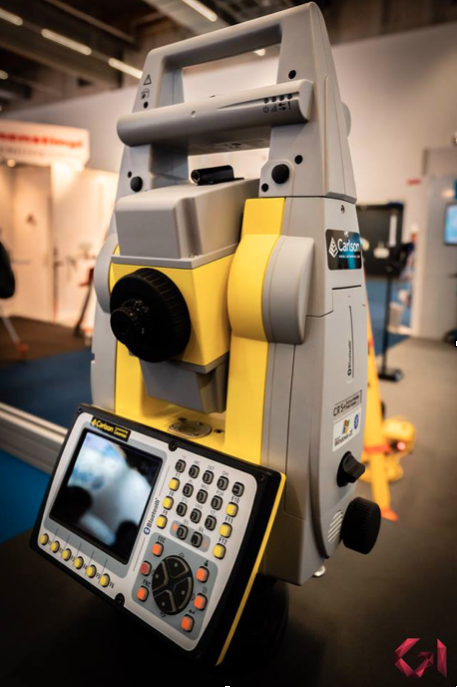
\includegraphics[width=0.2\textwidth]{figures/example}
            \caption{Robotic total station}
            \label{fig:example}
        \end{figure}
    \end{center}
    \section{Tables}\label{sec:tables}
    The tables should also be centered. The table description will be
    placed in front of the table and written in Arial, font size 10pt,
    bold, with 10pt~\cite{Durbin} blank space before and after. The description of
    the table will be labeled "Tab."~\ref{tab:example}.
    \begin{table}[!ht]
        \centering
        \begin{tabular}{|l|c|}
            \hline
            Column 1 & Column 2 \\
            \hline
            Monday & 1 \\
            Tuesday & 2 \\
            Wednesday & 3 \\
            Thursday & 4 \\
            Friday & 5 \\
            \hline
        \end{tabular}
        \caption{Working days}
        \label{tab:example}
    \end{table}
    \section{Example of equation numbering}\label{sec:equation}
    \begin{equation}
        a + b + c = d
    \end{equation}


% good linebraking of bibtex url
\setcounter{biburllcpenalty}{7000}
\setcounter{biburlucpenalty}{8000}

%% The bibliography
\printbibliography[heading=bibintoc]

\label{theend} % the last page of the thesis


\end{document}